\section{Testkonzept}\label{sec:testkonzept}

\subsection{Aufbau} \label{subsec:prinzip}

In der unteren Tabelle wird aufgeführt, welche Tests durchgeführt werden, um einen Überblick zu geben wie das Testkonzept aufgebaut ist. Die detaillierten Testprotokolle, die für die internen und externen Test verwendet werden, wird auf den Anhang verwiesen.  

\begin{figure}[H]
	\centering
	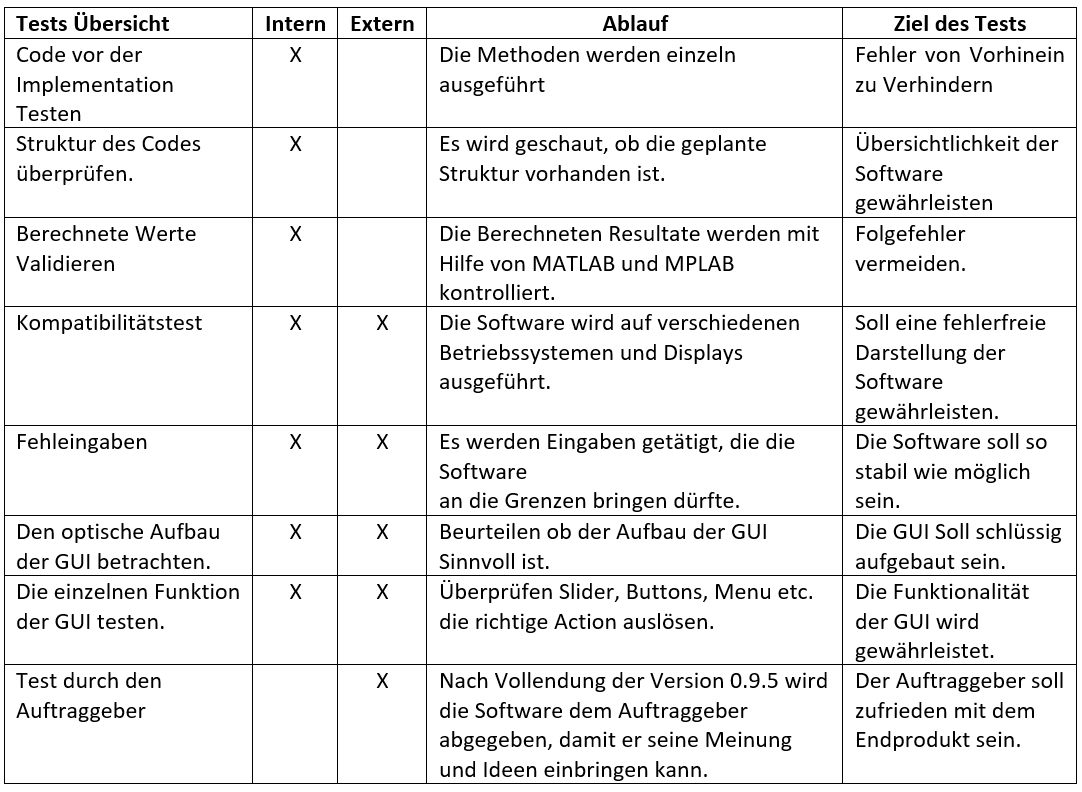
\includegraphics[width=16cm]{ueberblickTestKonzept.png}
	\label{fig:Test3}
\end{figure}

\begin{figure}[H]
	\centering
	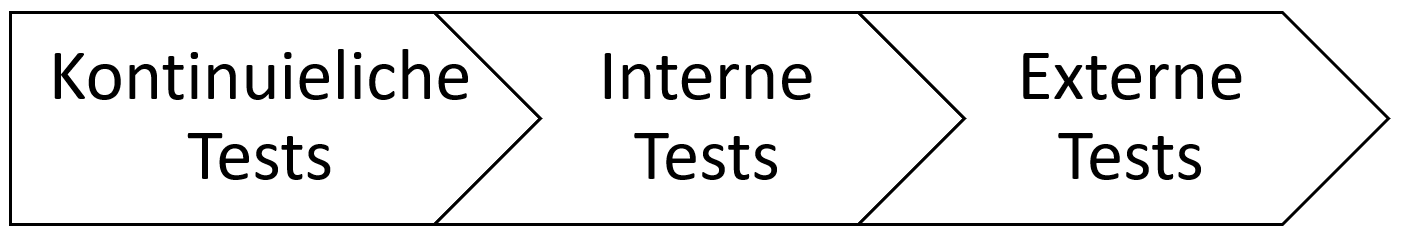
\includegraphics[width=16cm]{AblaufTestkonzept.png}
	\label{fig:Test3}
\end{figure}




\subsection{Validierung} \label{subsec:validierung}
Für die Berechnung des Insertionloss wird die Schaltung in mehreren Schritten vereinfacht. 
Die Zwischenschritte müssen auf ihre Korrektheit geprüft werden, um Folgefehler zu vermeiden, die wertvolle Zeit kosten können.
Diese werden mithilfe von mit Hilfe von MATLAB und MPLAB überprüft. 
Mit MATLAB werden die Rechenschritte noch einmal durchgeführt. Während in MPLAB die vereinfachte Schaltung Simuliert wird. Die erhaltenen Werte der beiden Tools werden miteinnader verglichen, ob sie übereinstimmen.  
 
\newpage
\subsection{Erwartungen} \label{subsec:validierung}
Die zu erwartenden Testresultate variieren stark von den Testperson, die die Software testet.
Die internen Tests werden die groben Fehler herausfiltern und schaffen eine stabile Grundlage auf die aufgebaut werden kann. Zudem wird überprüft, ob die alle Ziele erreicht wurden.
Bei den Fachpersonen wird das Feedback höchst wahrscheinlich sehr umfangreich   ausfallen. Es ist zu erwarten, dass Fehler entdeckt werden, die noch nicht bekannt sind oder die Software gar zum Absturz gebracht wird. 
Die Fachfremden Tester werden dies nicht erreichen, jedoch erhalten wir eine Hilfreiche Rückmeldung, was die Benutzerfreundlichkeit betrifft, weil diese Personen einen anderen Blick auf das grosse ganze haben. 
Das Feedback des Auftraggebers wird sehr detailliert ausfallen, weil er genaue Vorstellungen hat was er von dem Produkt haben möchte. Es wird sich, aber vermutlich mehrheitlich, um die Funktionen drehen und nicht welche Fehler es gibt. 





